Our study compares individuals who experienced the Reggio Approach with those who experienced other Northern Italian early childhood programs, as well as some who undertook no program at all. In this section, we document the Reggio Approach and explore the extent to which other early childhood programs in Reggio Emilia, Parma, and Padova implemented features of the Reggio Approach at different points of time.

\subsection{Municipal Early Childhood Schools of Reggio Emilia - The Reggio Approach}

Of the municipal systems in Reggio Emilia, Parma, and Padova, the Reggio Approach is notable for creative programming \textbf{[JJH: Innovative how? Please cut the bombast.][Edited to be more precise.]}, investment in staffing, early inclusion of children with disabilities, and high rates of provision of early childhood services. Of the three, Reggio Emilia was the first to develop a municipal early childhood system. It funds and manages the largest number of municipal infant-toddler and preschool sites.\footnote{Similar to Parma and Padova, Reggio Emilia contracts with local private providers and cooperatives to offer infant-toddler and preschool slots according to municipal regulations. These ``affiliated'' programs may not follow the Reggio Approach nor the municipal approaches in Parma and Padova. Accordingly, we consider this a separate sample during analysis.} 

In 1963, Reggio Emilia constructed its first municipal preschool for children aged 3-6 years; by 1975, the municipality offered 19 preschools \citep{Hohnerlein_2009_Paradox-Public-Preschools}. In 1965, the municipality legislated funding for infant-toddler centers for children aged 3 to 36 months. The first childcare site opened in 1971, and another 10 were added by 1979 \citep{Cagliari-etal-eds_2016_BOOK_Loris-Malaguzzi}. The municipal early childhood system in Reggio Emilia thus preceded Italy's key educational reforms of 1968 and 1971 which legislated free state preschools and local provision of infant-toddler childcare. \textbf{[JJH: Can we say that Reggio actually influenced reforms? Sylvi: I don't recommend saying this because Hohnerlein, a non-Reggio scholar, credits Bruno Ciari (and not Malaguzzi) for influencing the 1968 state reforms for public preschool. By citing the 2001 OECD report authored by FPGC scholar Rebecca New, however, we can state that Malaguzzi's influence came after the early 1970s, mainly in techniques to better engage families and in pedagogy (i.e., creativity as a vehicle for learning, use of pedagogistas, arts educators). The 2016 Malaguzzi book states that Reggio Emilia hosted 2 large conferences attended by 900 educators in the early 1970s to disseminate their new approaches throughout Italy. Shall we state this?]}

The Reggio Approach is a form of progressive early childhood education shaped by Loris Malaguzzi, a psychologist and educator influenced by Dewey's model of progressive education, Vygotsky, and the psychological theories of Piaget, Erikson, Bronfenbrenner, Bruner, and Gardner \citep{Rinaldi_2006_ReggioEmilia_BOOK,Cagliari-etal-eds_2016_BOOK_Loris-Malaguzzi} \textbf{[JJH: Do we know this? Please give me a citation. Talk is cheap and people rationalize what they did, see e.g., the Perry teacher survey. Did Reggio evolve? Gardner could not have had an effect. Sylvi: Regarding program evolution, according to the 2016 Malaguzzi book, the Reggio Approach features we reference in our survey were all in place by 1972. The book further cites the influence by the scholars listed above on Malaguzzi and the Reggio Approach. While Gardner came to Reggio after 1972, he provided teacher training and supported the use of creative arts in early childhood.]} Malaguzzi was also inspired by Bruno Ciari, who implemented Dewey's model in Bologna. Together, Ciari and Malaguzzi are credited with inciting a ``municipal school revolution'' in Italy by emphasizing learning, democratic participation, and social activism in early childhood, as an alternative to the welfare model and religious programming then-offered by the Catholic Church \citep{Lazzari_2012_Euro-J-Edu,Cagliari-etal-eds_2016_BOOK_Loris-Malaguzzi}.

In 1972, under Malaguzzi's direction, Reggio Emilia officially adopted Regulations for Municipal Schools that clarified the municipality's values for early childhood education, roles of parents and community members in municipal school management, staffing, professional development, enrollment priorities, and environmental features of preschools and infant-toddler centers \citep{Giaroni_1972_Regulations-Municipal-EC-Schools}. These regulations incorporate many of Ciari's innovations.\footnote{As director of municipal schools in Bologna from 1966-1970, Ciari promoted the physical learning environment, strong teacher-family relationships, participatory committees of parents and community members, and two co-teachers per classroom \citep{Edwards-etal-eds_1998_Hundred-Languages}.} 

From its inception, the engagement of families and the community was embedded in Reggio Approach practices. For example, parents and community members participate in school management to shape policies. Parents volunteer in classrooms and community members host field trips in the city \citep{CEHD_2016_Historical-Analysis,Cagliari-etal-eds_2016_BOOK_Loris-Malaguzzi}. To accommodate the needs of working parents, preschools and infant-toddler centers remain open five full-time days per week from September through June \citep{Giudici-Nicolosi_2014_Reggio-Approach}. Many municipal sites offer programming in July, and extended day options are available throughout the school year. To support all children in the community, Reggio Approach schools prioritize admission for children with disabilities and provide occupational, physical, and speech therapy as needed \citep{Edwards-etal-eds_1998_Hundred-Languages,Giaroni_1972_Regulations-Municipal-EC-Schools}.

In preschools, incoming 3-year-old cohorts form a homogenous classroom of about 25 children. Each cohort, according to municipal guidelines, are assigned two full-time co-teachers (teacher-pupil ratios are 1:12-13). \textbf{[JJH: Seems high! Sylvi: Compared to the US, it does seem high. Compared to Italy's state and religious schools, it was lower until the 2000s. We discuss this in the State subsection.]} At least one of the two teachers remains with each cohort for three consecutive years, offering extended time for continuity of care and strong teacher-family engagement. Each preschool site is also staffed by a full-time atelierista, an instructor with a background in visual arts, who helps teachers develop creative learning activities. On a biweekly basis, a pedagogista with a minimum bachelor's degree in psychology or pedagogy \textbf{[JJH: Post-BA? Be specific! Sylvi: Confirmed.]} supports the professional development for the educational staff of approximately 4-5 municipal preschools. Auxiliary site staff, such as cooks and janitors, are considered members of the educational team and participate in the biweekly trainings.\footnote{The Reggio Approach encouraged staffing of male educators in preschools from its inception. This policy conflicted with state law until 1978 \citep{Hohnerlein_2015_Development-and-Diffusion}.}

Reggio Approach environments reflect a light-filled, open interior design, furnished with natural materials and a garden. Each preschool is equipped with an atelier, or dedicated studio laboratory, where children and educators collaborate on creative instructional activities. In-house kitchens are surrounded by glass walls, to include children in the meal preparation process, and is used daily for preparing meals \citep{Rinaldi_2006_ReggioEmilia_BOOK,Vecchi_2010_ReggioEmilia_BOOK}. 

In Reggio Approach pedagogy, there is no institutionally-prescribed content knowledge that educators convey to children to achieve a specific academic goal, such as ``school readiness''. \textbf{[Team: The preceding sentence includes minor edits for preciseness.]} Instead, curriculum is viewed as an ongoing, collaborative project between educators, children and families. Learning goals are determined by children and adults, and achieved through creative long-term projects with flexible timelines. Thus, teachers and children are jointly viewed as researchers and co-creators of knowledge. For example, adults and children collaborate to define a question or topic. Learning is then pursued following a scientific process: theories are shared, tested, and revised through socratic questions and dialogue. \textbf{[JJH: Reggio's curriculum is more method than content (in contrast to state, religious, and the other municipal programs which emphasize content). But this is not shared by other schools? How do we know? Sylvi: We asked two questions about this in our survey to evaluate exactly this. Further, the ECE scholar who collected survey data in Padova on our behalf confirmed.]} Teachers observe children's development, listen, interact with children through questions and dialogue, and provide scaffolding to extend learning. Children demonstrate their emerging knowledge through expressive art forms, with aid from the atelierista. Teachers organize each child's documented work in a portfolio that is shared with children and parents over the year to observe the child's development \citep{Rinaldi_2006_ReggioEmilia_BOOK,Giudici-Nicolosi_2014_Reggio-Approach}.

\subsection{Comparison of Early Childhood Programs in Northern Italy: 1950-2010}

Capturing lifecycle treatment effects from the Reggio Approach depends on the degree to which early childhood programs attended by comparison groups share similar practices. To the extent that these programs overlap, it is reasonable to expect lower treatment effects from comparisons of those who attend any program, than from comparisons with individuals who attended no early childhood program. 

To increase our understanding of the available early childhood systems besides the Reggio Approach, and how each evolved from 1950 through 2010, we administered an original survey to current and former educational coordinators and school administrators in Reggio Emilia, Parma, and Padova. The survey was designed to explore the extent to which the key administrative and pedagogical components of the Reggio Approach were present in each city's municipal, state, and religious early childhood programs at different points of time \citep{CEHD_2016_Historical-Analysis}. 

To confirm the results of our survey and document provision and enrollment in each of the available early childhood systems, we further collected administrative data from historical archives in Reggio Emilia and Padova. We were unsuccessful in sourcing similar records from Parma \citep{Padova-Admin-Data_1964-2011,Reggio-Admin-data_1966-2006,Reggio-Annual-Journals_1994-2011}. 

\textbf{[JJH: Earlier we say we have no historical data on Parma -- now suddenly we do. Which is correct? Sylvi: The above has been edited to clarify the distinction that Parma's municipal system DID respond to our survey as indicated in Table 1. We could not, however, retrieve administrative data from Parma's municipal archives.]}

Together, survey results and administrative data indicate that educational preschool became available to each cohort in each of the various systems as listed in Table~\ref{tab:pre}. 

\begin{table}[H]
\centering
\caption{Availability of Preschool Programs by City and School Type}\label{tab:pre}
\begin{adjustbox}{width=\textwidth}
\begin{threeparttable}
	\begin{tabular}{l l c c c c c c c c c}
\toprule
\mc{1}{c}{Cohort} & \mc{1}{c}{Years} & \mc{3}{c}{Reggio Emilia} & \mc{3}{c}{Parma} & \mc{3}{c}{Padova} \\
& & Municipal & Catholic & State & Municipal & Catholic & State & Municipal & Catholic & State \\
\midrule
Adults 50s & 1957-1965 & & \checkmark & & & \checkmark & & & \checkmark & \\
Adults 40s & 1972-1976 & \checkmark & \checkmark & & & \checkmark & & & \checkmark & \\
Adults 30s & 1983-1987 & \checkmark & \checkmark & \checkmark & \checkmark & \checkmark & \checkmark & \checkmark & \checkmark & \checkmark \\
Adolescents & 1994-2000 & \checkmark & \checkmark & \checkmark & \checkmark & \checkmark & \checkmark & \checkmark & \checkmark & \checkmark \\
Children & 2009-2014 & \checkmark & \checkmark & \checkmark & \checkmark & \checkmark & \checkmark & \checkmark & \checkmark & \checkmark \\
\bottomrule
\end{tabular}

% Caption:
% Note: This table indicates the types of educational preschool systems (defined as programs with 4 or more sites) available to parents in each city during the years each cohort was eligible for a 3-6 year old program. 
\begin{tablenotes}
Note: This table indicates the provision by system of educational preschool systems (defined as programs with 4 or more sites) available in each city during the years each cohort was eligible to attend a 3-6 year old program. 
\end{tablenotes}
\end{threeparttable}
\end{adjustbox}
\end{table}

The survey includes key pedagogical and administrative features of the Reggio Approach. Selected components were identified by published program descriptions and confirmed by scholars of the Reggio Approach and early childhood programs in Northern Italy.\footnote{See \citet{Edwards-etal-eds_1998_Hundred-Languages} and \citet{Corsaro_2008_Policy-Practice}.} The list of components includes aspects of administrative program operations such as staffing, supervision, enrollment, and funding. It also considers pedagogy and educational practices for children's learning and parental engagement. Respondents were asked to indicate whether these central features of the Reggio Approach were present in their systems during different decades. Additional questions were included to understand (i) the extent of variation between municipal programs and private providers contracted by the municipality; (ii) the extent of site-level variation within systems; (iii) the perceived variation between similar systems in other cities; (iv) the sources of program funding, and (v) the services available for immigrant families. See Appendix~\ref{sec:survey} for the full survey. 

\subsubsection{Survey Results}

Table~\ref{tab:respondents} identifies the school systems in each city that completed our survey. We acknowledge that the small sample of survey respondents may be too limited to ensure reliable reporting of representative results. Despite this, the responses are useful for presenting information that is not readily available in published literature.

\begin{table}[H]
\centering
\caption{Survey Respondents by City and School Type}\label{tab:respondents}
\begin{threeparttable}
	\begin{tabular}{lccc}
\toprule
City & Municipal & State & Religious \\
\midrule
Reggio Emilia & \checkmark & \checkmark & \\
Parma		& \checkmark & & \\
Padova & \checkmark & \checkmark & \checkmark \\
\bottomrule
\end{tabular}
\begin{tablenotes}
\footnotesize Note: This table indicates the systems represented by survey respondents. These individuals include current and former administrators and educational coordinators. One survey was administered for each system noted. Answers reflect the input of multiple people associated with the system. Responses were provided by religious systems in Reggio Emilia and Parma; we do not report them here as they are incomplete. \end{tablenotes}
\end{threeparttable}
\end{table}

\textbf{[JJH: Flatten table.][Edited]}

Overall, results from the survey indicate that early childhood education systems within Reggio Emilia, as well as in Parma and Padova, share a number of characteristics. The general trend shows that programming and practices endorsed by the municipality of Reggio Emilia are present in other early childhood systems, albeit to different degrees and at different times. 

We first compare the different programs in Figures~\ref{fig:agg-admin} and~\ref{fig:agg-ped}. We examine 14 administrative components and 16 pedagogical components (not all of the pedagogical components were present in the Reggio Approach). Using survey results, we calculate the number of administrative and pedagogical components that each program shared with the Reggio Approach by school type, city, and year. The evidence indicates that, over time, non-Reggio Approach programs increasingly implemented more of the pedagogical and administrative practices endorsed by the Reggio Approach. This is especially true for Parma's municipal program, and to a lesser extent for Padova's municipal program. State and religious systems systems report implementing more administrative practices endorsed by the Reggio Approach than pedagogical components. 

\begin{figure}[H]
\begin{center}
\begin{subfigure}[b]{0.49\textwidth}
	\caption{Number of Administrative Characteristics in Common with the Reggio Approach}\label{fig:agg-admin}
	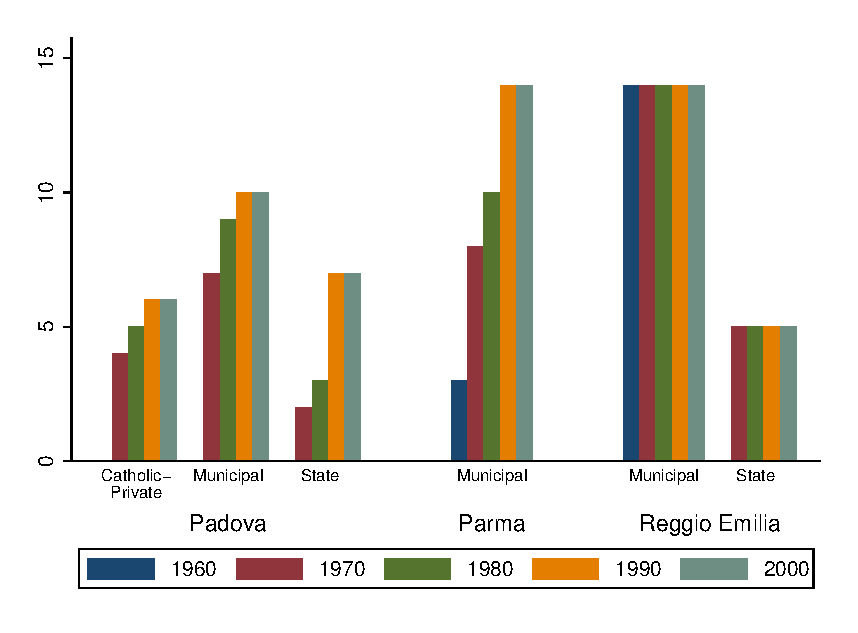
\includegraphics[width=\textwidth]{../../output/aggregateAdministrative.eps}
\end{subfigure}%
~
\begin{subfigure}[b]{0.49\textwidth}
	\caption{Number of Pedagogical Characteristics in Common with the Reggio Approach}\label{fig:agg-ped}
	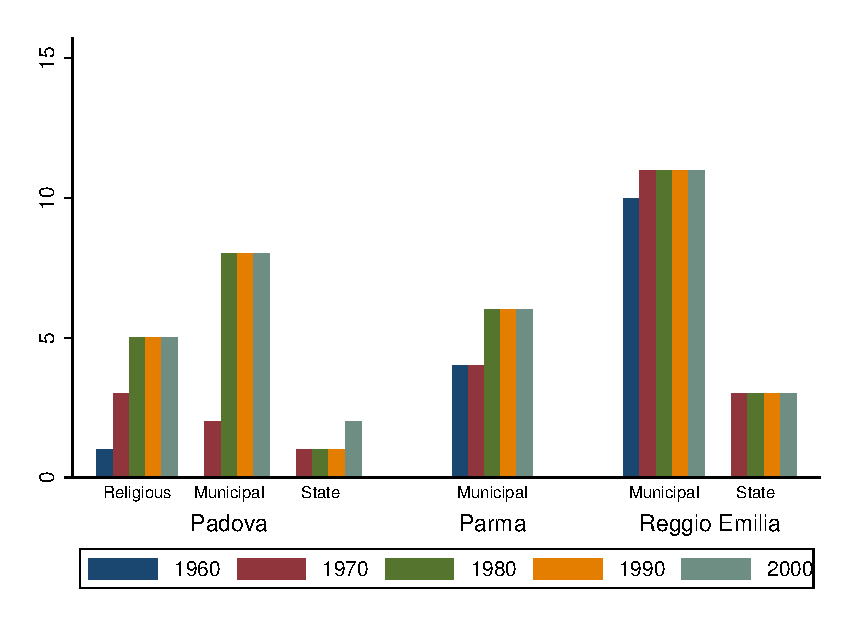
\includegraphics[width=\textwidth]{../../output/aggregatePedagogical.eps}
\end{subfigure}%
\end{center}
\raggedright \footnotesize Note: These graphs show the number of administrative and pedagogical components that each program has in common with the Reggio Approach. We consider 14 administrative components and 16 pedagogical components. Some of the pedagogical components were not present in the Reggio Approach.
\end{figure}

\textbf{[JJH: Can we put in color?] [Typist: Professor, these are currently in color. We will print you a color version tonight.]}
\textbf{[JJH: Please break out the pedagogical components --- summing conceptually different items is a meaningless exercise. Team: This is added below.]}

While the Reggio Approach remains distinctive when considering the combination of its elements, the alternative systems surveyed in our study evolved to include a substantial portion of the elements in Reggio Emilia's municipal system. To better understand which features of the Reggio Approach were adopted by other programs and how they evolved, we document key components by decade and by each system in Tables~\ref{tab:survey-data-atrisk} to~\ref{tab:survey-data-ped}. For the full set of survey items and responses, see Appendix~\ref{sec:survey}.

\begin{table}[H]
	\caption{Policies to Support At-Risk Children and Working Families}\label{tab:survey-data-atrisk}
\centering
\begin{threeparttable}
\begin{tabular}{L{4.5cm} c c c c c c c}
\toprule																	
	&		&	\mc{2}{c}{Reggio Emilia}	&	Parma &	\mc{3}{c}{Padova}	\\	
	\cmidrule(lr){3-4} \cmidrule(lr){5-5} \cmidrule(lr){6-8}
& & Municipal & State & Municipal & Municipal & State & Religious \\
\midrule
\multirow{5}{4.5cm}{Preschools are open 8 hours daily} 	&	1960	&	\checkmark	&		&	\checkmark	&		&		&		\\	
		&	1970	&	\checkmark	&	\checkmark	&	\checkmark	&	\checkmark	&	\checkmark	&	\checkmark	\\	
		&	1980	&	\checkmark	&	\checkmark	&	\checkmark	&	\checkmark	&	\checkmark	&	\checkmark	\\	
		&	1990	&	\checkmark	&	\checkmark	&	\checkmark	&	\checkmark	&	\checkmark	&	\checkmark	\\	
		&	2000	&	\checkmark	&	\checkmark	&	\checkmark	&	\checkmark	&	\checkmark	&	\checkmark	\\	\midrule
\multirow{5}{4.5cm}{Program sites offer extended hours for working families}	&	1960	&	\checkmark	&		&	\checkmark	&		&		&		\\	
		&	1970	&	\checkmark	&	\checkmark	&	\checkmark	&	\checkmark	&		&	\checkmark	\\	
		&	1980	&	\checkmark	&	\checkmark	&	\checkmark	&	\checkmark	&		&	\checkmark	\\	
		&	1990	&	\checkmark	&	\checkmark	&	\checkmark	&	\checkmark	&		&	\checkmark	\\	
		&	2000	&	\checkmark	&	\checkmark	&	\checkmark	&	\checkmark	&		&	\checkmark	\\	\midrule
\multirow{5}{4.5cm}{Priority of enrollment is given to economically disadvantaged families}	&	1960	&	\checkmark	&		&	\checkmark	&		&		&		\\	
		&	1970	&	\checkmark	&	\checkmark	&	\checkmark	&	\checkmark	&		&		\\	
		&	1980	&	\checkmark	&	\checkmark	&	\checkmark	&	\checkmark	&		&		\\	
		&	1990	&	\checkmark	&	\checkmark	&	\checkmark	&	\checkmark	&		&		\\	
		&	2000	&	\checkmark	&	\checkmark	&	\checkmark	&	\checkmark	&		&		\\	\midrule
\multirow{5}{4.5cm}{Priority of enrollment is given to children with disabilities}	&	1960	&	\checkmark	&		&		&		&		&		\\	
		&	1970	&	\checkmark	&	\checkmark	&		&	\checkmark	&	\checkmark	&		\\	
		&	1980	&	\checkmark	&	\checkmark	&		&	\checkmark	&	\checkmark	&		\\	
		&	1990	&	\checkmark	&	\checkmark	&	\checkmark	&	\checkmark	&	\checkmark	&	\checkmark	\\	
		&	2000	&	\checkmark	&	\checkmark	&	\checkmark	&	\checkmark	&	\checkmark	&	\checkmark	\\	\midrule
\multirow{5}{4.5cm}{Priority of enrollment is given to single-parent families}	&	1960	&	\checkmark	&		&		&		&		&		\\	
		&	1970	&	\checkmark	&		&		&	\checkmark	&		&		\\	
		&	1980	&	\checkmark	&		&	\checkmark	&	\checkmark	&		&		\\	
		&	1990	&	\checkmark	&		&	\checkmark	&	\checkmark	&	\checkmark	&		\\	
		&	2000	&	\checkmark	&		&	\checkmark	&	\checkmark	&	\checkmark	&		\\	
\bottomrule	
\end{tabular}	
\end{threeparttable}																
\end{table}

\begin{table}[H]
	\caption{Administrative Practices}\label{tab:survey-data-admin}
\centering
\begin{adjustbox}{width=0.9\textwidth}
\begin{threeparttable}
\begin{tabular}{L{5cm} c c c c c c c}
\toprule																	
	&		&	\mc{2}{c}{Reggio Emilia}	&	Parma &	\mc{3}{c}{Padova}	\\	
	\cmidrule(lr){3-4} \cmidrule(lr){5-5} \cmidrule(lr){6-8}
& & Municipal & State & Municipal & Municipal & State & Religious \\
\midrule
\multirow{5}{5cm}{Parental boards or advisory groups are encouraged as active participants in school culture}	&	1960	&	\checkmark	&		&		&		&		&		\\	
	&	1970	&	\checkmark	&	\checkmark	&	\checkmark	&	\checkmark	&		&	\checkmark	\\	
	&	1980	&	\checkmark	&	\checkmark	&	\checkmark	&	\checkmark	&		&	\checkmark	\\	
	&	1990	&	\checkmark	&	\checkmark	&	\checkmark	&	\checkmark	&		&	\checkmark	\\	
	&	2000	&	\checkmark	&	\checkmark	&	\checkmark	&	\checkmark	&		&	\checkmark	\\ \midrule
\multirow{5}{5cm}{Full-time, degreed Pedagogistas\footnote{In non-Reggio Approach systems, this role is referred to as Educative Coordinator. The job responsibilities of Educative Coordinators do vary across cities and ECE systems.} are hired by the system to oversee professional development for multiple program sites}	&	1960	&	\checkmark	&		&		&		&		&		\\	
	&	1970	&	\checkmark	&		&		&		&		&		\\	
	&	1980	&	\checkmark	&		&		&	\checkmark	&		&		\\	
	&	1990	&	\checkmark	&		&	\checkmark	&	\checkmark	&	\checkmark	&		\\	
	&	2000	&	\checkmark	&		&	\checkmark	&	\checkmark	&	\checkmark	&		\\	\midrule
\multirow{5}{5cm}{Professional development is provided by highly trained educational coordinators to each program site every 1-2 weeks\footnote{In Padova's religious programs, professional development is provided by a mixture of part-time and full-time Educative Coordinators.}}	&	1960	&	\checkmark	&		&		&		&		&		\\	
	&	1970	&	\checkmark	&		&		&		&		&	\checkmark	\\	
	&	1980	&	\checkmark	&		&		&		&		&	\checkmark	\\	
	&	1990	&	\checkmark	&		&	\checkmark	&		&	\checkmark	&	\checkmark	\\	
	&	2000	&	\checkmark	&		&	\checkmark	&		&	\checkmark	&	\checkmark	\\	\midrule
\multirow{5}{5cm}{Full-time Atelierista, or expert in creative visual arts, is staffed at each preschool site and collaborates with classroom teachers to design creative learning activities}
	&	1960	&	\checkmark	&		&		&		&		&		\\	
	&	1970	&	\checkmark	&		&		&		&		&		\\	
	&	1980	&	\checkmark	&		&		&	\checkmark	&		&		\\	
	&	1990	&	\checkmark	&		&		&	\checkmark	&		&		\\	
	&	2000	&	\checkmark	&		&		&	\checkmark	&		&		\\	\midrule
\multirow{5}{5cm}{Kitchen and janitorial staff join educators for professional development}	&	1960	&	\checkmark	&		&		&		&		&		\\	
	&	1970	&	\checkmark	&		&	\checkmark	&		&		&		\\	
	&	1980	&	\checkmark	&		&	\checkmark	&		&		&		\\	
	&	1990	&	\checkmark	&		&	\checkmark	&		&		&		\\	
	&	2000	&	\checkmark	&		&	\checkmark	&	\checkmark	&		&		\\	\midrule
\multirow{5}{5cm}{Scheduled work hours are set aside weekly for teachers to document children's work}	&	1960	&	\checkmark	&		&		&		&		&		\\	
	&	1970	&	\checkmark	&		&		&	\checkmark	&		&		\\	
	&	1980	&	\checkmark	&		&	\checkmark	&	\checkmark	&		&	\checkmark	\\	
	&	1990	&	\checkmark	&		&	\checkmark	&	\checkmark	&		&	\checkmark	\\	
	&	2000	&	\checkmark	&		&	\checkmark	&	\checkmark	&		&	\checkmark	\\	\midrule
\multirow{5}{5cm}{Scheduled hours are set aside weekly for teachers to engage families}	&	1960	&	\checkmark	&		&		&		&		&		\\	
	&	1970	&	\checkmark	&		&	\checkmark	&		&		&	\checkmark	\\	
	&	1980	&	\checkmark	&		&	\checkmark	&		&		&	\checkmark	\\	
	&	1990	&	\checkmark	&		&	\checkmark	&	\checkmark	&		&	\checkmark	\\	
	&	2000	&	\checkmark	&		&	\checkmark	&	\checkmark	&		&	\checkmark	\\	\midrule
\multirow{5}{5cm}{Classrooms are homogeneous in age} 	&	1960	&	\checkmark	&		&		&		&		&		\\	
	&	1970	&	\checkmark	&	\checkmark	&		&		&		&		\\	
	&	1980	&	\checkmark	&	\checkmark	&		&		&		&		\\	
	&	1990	&	\checkmark	&	\checkmark	&		&		&		&		\\	
	&	2000	&	\checkmark	&	\checkmark	&		&		&		&		\\	\midrule
\multirow{5}{5cm}{2 co-teachers for incoming cohorts of 3 year olds. At least 1 teacher stays with the cohort for the next two years to maintain continuity of care}	&	1960	&		&		&		&		&		&		\\	
	&	1970	&	\checkmark	&	\checkmark	&		&		&		&		\\	
	&	1980	&	\checkmark	&	\checkmark	&	\checkmark	&	\checkmark	&		&		\\	
	&	1990	&	\checkmark	&	\checkmark	&	\checkmark	&	\checkmark	&		&		\\	
	&	2000	&	\checkmark	&	\checkmark	&	\checkmark	&		&		&		\\	
\bottomrule
\end{tabular}
\end{threeparttable}		
\end{adjustbox}															
\end{table}

\begin{table}[H]
	\caption{Pedagogical Components}\label{tab:survey-data-ped}
\centering
\begin{adjustbox}{width=\textwidth}
\begin{threeparttable}
\begin{tabular}{L{5.5cm} c c c c c c c}
\toprule																	
	&		&	\mc{2}{c}{Reggio Emilia}	&	Parma &	\mc{3}{c}{Padova}	\\	
	\cmidrule(lr){3-4} \cmidrule(lr){5-5} \cmidrule(lr){6-8}
& & Municipal & State & Municipal & Municipal & State & Religious \\
\midrule
\multirow{5}{5.5cm}{Theories of psychology and early childhood education (e.g. Bloom, Bruner, Gardner, Piaget, Vygotsky) influenced educational approaches}	&	1960	&	\checkmark	&		&		&		&		&		\\	
		&	1970	&	\checkmark	&		&		&		&		&		\\	
		&	1980	&	\checkmark	&		&	\checkmark	&	\checkmark	&		&	\checkmark	\\	
		&	1990	&	\checkmark	&		&	\checkmark	&	\checkmark	&		&	\checkmark	\\	
		&	2000	&	\checkmark	&		&	\checkmark	&	\checkmark	&		&	\checkmark	\\	\midrule
\multirow{5}{5.5cm}{Curriculum emerges through research-based projects with unlimited timelines}	&	1960	&	\checkmark	&		&		&		&		&		\\	
		&	1970	&	\checkmark	&		&		&		&		&		\\	
		&	1980	&	\checkmark	&		&		&	\checkmark	&		&		\\	
		&	1990	&	\checkmark	&		&	\checkmark	&	\checkmark	&		&		\\	
		&	2000	&	\checkmark	&		&	\checkmark	&	\checkmark	&		&		\\	\midrule
\multirow{5}{5.5cm}{Visual arts help children learn}	&	1960	&	\checkmark	&		&	\checkmark	&		&		&	\checkmark	\\	
		&	1970	&	\checkmark	&		&	\checkmark	&		&		&	\checkmark	\\	
		&	1980	&	\checkmark	&		&	\checkmark	&		&		&	\checkmark	\\	
		&	1990	&	\checkmark	&		&	\checkmark	&		&		&	\checkmark	\\	
		&	2000	&	\checkmark	&		&	\checkmark	&		&		&	\checkmark	\\	\midrule
\multirow{5}{5.5cm}{Teachers document children's learning}	&	1960	&	\checkmark	&		&		&		&		&		\\	
		&	1970	&	\checkmark	&		&		&	\checkmark	&		&	\checkmark	\\	
		&	1980	&	\checkmark	&		&	\checkmark	&	\checkmark	&		&	\checkmark	\\	
		&	1990	&	\checkmark	&		&	\checkmark	&	\checkmark	&		&	\checkmark	\\	
		&	2000	&	\checkmark	&		&	\checkmark	&	\checkmark	&	\checkmark	&	\checkmark	\\
	\bottomrule
\end{tabular}	
\end{threeparttable}	
\end{adjustbox}															
\end{table}					

These results indicate that the main components of the Reggio Approach practiced in non-Reggio Approach programs include (i) the engagement of families in school management; (ii) administrative practices for at-risk children and working families, and; (iii) the use of highly trained educational coordinators to routinely support professional development. In general, non-Reggio Approach programs are similar to each other, and different from the Reggio Approach, in providing religious teaching and following a daily program designed to guide children in acquiring knowledge of specific concepts. 

The general trend is consistent with the explanation that common influences were operating at the onset of these programs. Additionally, survey results mildly support a spillover story of Reggio Approach features into other early childhood programs as treatment effects are found only for the oldest cohorts. We more closely examine these patterns in each of the other early childhood systems below. 

\textbf{[JJH: How can a survey reveal spillovers or not? Team: We cannot definitely state there is spillover. The text has been edited to reflect this.]} 

\subsection{State Preschools}

Over time and across cities, each cohort in our sample had access to different numbers of state preschools. Further, those who enrolled in state programs experienced varying early childhood curricula and administrative practices.

In 1968, Law 444 ensured access to a system of free, state preschool for all families that applied.\footnote{In state programs, parents pay only for meals and transportation.} Law 444 is considered a key shift in Italian policies for early childhood as it legitimized state involvement in public and private education for ages 3-6 years \citep{Hohnerlein_2009_Paradox-Public-Preschools}. \textbf{[JJH: Discuss features of the 1968 literature. Sylvi: This is added.]} By Law 444, the state was responsible for school construction, materials and equipment. Municipalities, however, were mandated to maintain state preschools and fund the salaries of an all-female teaching staff under 35 years of age, with a vocational diploma from a 3-year high school \citep{OECD_2001_Italy-Country-Note}.\footnote{Later reforms transferred constructions costs from the state to municipalities, allowed men to work as early childhood educators, and required laureate degrees.} 

By providing funds only to construct state preschools where local demand was not met by existing non-state systems such as municipal and religious schools, Law 444 resulted in disparate numbers of state preschools in Reggio Emilia, Parma, and Padova for each of the cohorts in our evaluation \citep{Hohnerlein_2009_Paradox-Public-Preschools}. Historical records indicate that state preschools first appeared in Reggio Emilia and Padova between 1973-1975 \citep{Padova-Admin-Data_1964-2011,Reggio-Admin-data_1966-2006,Reggio-Annual-Journals_1994-2011}. In contrast to other areas of Italy where the state is currently the largest provider of preschool education, enrollment in Reggio Emilia, Parma, and Padova's state preschools is historically lower than enrollment in municipal and religious preschools. Although the state does not offer infant-toddler childcare, it regulates and subsidizes these programs through regional governments per Law 1044 enacted in 1971.

\textbf{[JJH: What is municipal and what is municipal preschool? Team: we use ``system'' to indicate the network of infant-toddler and preschool sites. We have clarified the above sentence to read preschool instead of program.]}

Reports suggest that periodic policy reforms and improved guidelines for state preschools (Orientamenti) were influenced by municipal programs from the region of Emilia Romagna, including Reggio Emilia, Milan, and Pistoia \citep{OECD_2001_Italy-Country-Note}. In particular, revised mandates for lower teacher-child ratios, and higher qualifications for teacher education are proposed as key quality indicators associated with diminishing disparities in state and non-state programs by the end of the 20th century \citep{Hohnerlein_2015_Development-and-Diffusion}. For example, between 1969 and 1980 for the age-40 and age-30 cohorts, teacher-child ratios were very low ranging from 1:17-30 children aged 3-6 years, and teacher education took place in religious institutions.\footnote{In contrast, teacher-child ratios in the Reggio Approach were 2:25-30 from 1972 forward.} After 1991, attendees of state preschools in the adolescent and child cohorts experienced better physical accessibility to schools, a 1:12-13 teacher-child ratio (equivalent to that of the Reggio Approach), and teachers who were trained in universities \citep{Hohnerlein_2015_Development-and-Diffusion}. The two younger cohorts further benefitted from 1991 revisions to Orientamenti stressing the contributions of social relationships for cognitive development and the value of communication for home-school relationships \citep{OECD_2001_Italy-Country-Note}. Six content goals for early childhood education and their associated skill-sets were also outlined by the state for the first time, including (i) the body and movement; (ii) language and speech; (iii) space, order, and measure; (iv) things, time, and nature; (v) messages, forms and media, and; (vi) the self and other \citep{Orientamenti_1991_Scuola-Materna}.\footnote{In the Reggio Approach, specific skill-sets to be acquired are explicitly not stated as a requirement for early childhood education.} The methods, however, by which these concepts should be taught were not stated in order to enable autonomy and flexibility at the school-level.

In theory, mandated administrative operations and policies for state preschools should be consistent throughout Italy. Indeed, survey results indicate that administrative operations for state preschools in Padova are similar to state preschools in Reggio Emilia, with two interesting exceptions. In Padova, parents must pay for extras such as field trips, whereas in Reggio Emilia, field trips for children in state preschools are funded by the municipality. Padova's state preschools report staffing full-time educational coordinators to provide professional development for state teachers from the 1990s forward, which is a feature of the Reggio Approach. In Reggio Emilia, however, state preschools do not report the hiring of full-time educational coordinators. 

Survey results indicate that several administrative features of state preschools are different from the Reggio Approach (and from municipal programs in Parma and Padova). State preschools do not hire a full-time expert in the creative arts and do not set aside time for teachers to engage families. State preschools do not offer extended hours to working families. And, at 30 hours per week, state teachers work 6 hours less than their municipal counterparts. With reduced teaching hours and reduced full-time staff, children in state preschools spend more hours with only one teacher than do children in Reggio Approach preschools (see Appendix Table \ref{tab:programoperation}). 

In support of a spillover argument, state preschools in Reggio Emilia implement two Reggio Approach practices that are not offered in Padova's state preschools. These practices include the use of homogeneous-aged classrooms and the focus on continuity of care for children and families by keeping at least one teacher with each cohort for three years. Overall, however, pedagogy in state preschools of both Reggio Emilia and Padova  supports children's learning differently than in the Reggio Approach. State preschools (like religious preschools in all three cities) emphasize moral development, national patriotism and family values. Survey results further indicate that teaching in state preschools (like municipal schools in Parma and Padova), is influenced by different academic theories, includes religious teaching, and use programmed daily activities to guide children in learning of specific concepts (see Appendix Tables~\ref{tab:programoperation} to \ref{tab:environ-features}). 

Our study evaluated whether these additional features of Reggio have any benefits. They appear not to. \textbf{[Team: We propose the following revision: Our study evaluated whether features of the Reggio Approach not employed by state preschools were effective in benefitting individuals sufficiently to cause significant improvement in outcomes relative to individuals who did not receive the Reggio Approach. They appear not to.]}

\subsection{Religious Early Childhood Programs}

The Catholic Church is the oldest early childhood provider in Italy, offering both religious training and charitable social services for disadvantaged children since the 19th century \citep{OECD_2001_Italy-Country-Note}. All five cohorts in our evaluation had access to religious programming for ages 3-6 years; of the three cities, Padova offers the largest number of religious preschools. Until the 1990s, religious sites in Reggio Emilia, Parma, and Padova did not offer educational infant-toddler programs. At some sites in each municipality, the adolescent cohort had access to several months of transitional programming for children over 24 months of age; from 12 months of age, the child cohort had access to infant-toddler childcare \citep{Malizia-Cicatelli_2011_BOOK_Catholic-School,CEHD_2016_Historical-Analysis}.

To provide administrative support for independent religious schools, local federations began to assemble throughout Italy in the mid-1970s. Religious preschools within the cities of Reggio Emilia, Parma, and Padova could join a city-level federation that supported administrative operations. \textbf{[JJH: Churches? What's a site? Church? Sylvi: Correct. JJH: What is the content of the program? Sylvi: We revised the text below to reflect educational goals for equitable religious schools for cohorts after 1997-2000. Before then, none are reported in the literature nor in our survey. For all of our cohorts, however, there is no stated pedagogical approach to achieve these stated goals that we can ascribe to individual religious sites nor to local federations such as the use of project-based active-child learning or teacher-initiated activities.]} In contrast to the Reggio Approach, however, religious schools within the same local federation are not mandated to implement a unified pedagogy for preschool education; in this sense, the Church supports the autonomy of individual religious sites to determine their own methodologies \citep{Malizia-Cicatelli_2011_BOOK_Catholic-School}. 

Following a 1997 policy that enabled state funding for non-state programs meeting national guidelines for early childhood, the Catholic Church undertook significant efforts to quantify and achieve equitable program quality in religious schools for all ages. At some time after 1997, we can expect that policies and educational goals in religious preschools seeking equitable status began to reflect state laws and guidelines. Indeed, after 2000, the Church reports efforts throughout Italy to replace religious educators with secular teachers trained in higher institutions and reducing teacher-child ratios to reflect national standards \citep{Malizia-Cicatelli_2011_BOOK_Catholic-School}. Religious programs that succeeded in achieving equitable status would thus, like state preschools, reflect the influence of municipal systems in the Province of Emilia Romagna, including Reggio Emilia \citep{Hohnerlein_2009_Paradox-Public-Preschools,OECD_2001_Italy-Country-Note}. 

Our study does not collect site-level data that would confirm which religious early childhood programs achieved equitable status nor the timing of such a shift; we cannot thus determine the extent to which adolescents and children in our evaluation may have attended equitable religious schools. Survey results indicate that the majority of religious sites in all three municipalities achieved equitable status during the 2000s. We thus estimate that the child cohort likely had access to equitable religious preschools; those children who enrolled experienced a program of similar quality as children who enrolled in state preschools. We further note that parents of the youngest cohort who chose equitable religious preschools were eligible for subsidized tuition on a sliding-scale basis; prior to 2000, tuition and fees for religious preschool in all three cities was more expensive than the cost of attending municipal and state preschools.

Survey results for religious preschools are available for Reggio Emilia for the 2000s, reflecting only the experience of the child cohort in our study. In support of a spillover story, religious preschools in Reggio Emilia are the only other system we survey that do not implement daily activities to guide children in acquiring specific content knowledge. Religious preschools in Reggio Emilia, further like the Reggio Approach and unlike religious preschools in Padova, hire full-time educational coordinators, keep at least one of two co-teachers with each cohort for three years to ensure continuity of care, and maintain homogenous-aged classrooms.\footnote{Survey results indicate that homogenous-aged classrooms are only practiced in Reggio Emilia; all systems in Parma and Padova maintain mixed-age classrooms.} Religious preschools in Reggio Emilia, like the Reggio Approach, also offer extended hours for working families; include an atelier, in-house kitchen, and emphasize natural materials and open spaces; encourage parents to serve on school boards; hire full-time educational coordinators to oversee professional development; are influenced by the same academic theories; employ project-based learning with flexible timelines; set weekly hours for teachers to engage families and document children's work; and incorporate fine arts to support children's learning. 

Of all the systems we survey, only Padova's religious early childhood system reports that Malaguzzi's educational practices shaped their daily program; this influence is reported only for some religious sites starting in the 2000s. Regardless, survey evidence suggests that religious preschools in Padova share the following practices with the Reggio Approach: from the 1970s, schools were open 8 hours and extended hours were available for working parents; parents were encouraged to serve on school boards and weekly time was set aside for teachers to engage families. From the 1980s, teachers began to document children's work and school environments included an atelier. From the 1990s, Padova's religious schools prioritized enrollment for children with disabilities. 

Unlike the Reggio Approach, pedagogy in both systems include religious teaching; an emphasis on moral development, national patriotism and family values, and; the influence of Agazzi, Froebl and Montessori. Only Padova's religious preschools follow a daily program to guide children in learning specific concepts (see Appendix Table \ref{tab:educ-program}). Municipal archives from 1970 indicate that children aged 3-6 years enrolled in Padova's religious preschools experienced one teacher for 34-44 children \citep{Padova-Admin-Data_1964-2011}. 

Unlike the Reggio Approach, religious preschools in Reggio Emilia and Padova do not prioritize the enrollment of children from economically disadvantaged families (see Appendix Table \ref{tab:administrative-atrisk}).  In Reggio Emilia only, religious preschools are not open 8 hours daily; do not hire full-time atelieristas; do not include cooks and janitors in teacher trainings, and; do not provide teachers with supervision and training on a biweekly basis. These components appear to have no effects for the outcomes that we study.

\subsection{Municipal Early Childhood Systems in Parma and Padova}

\textbf{[JJH: This section is very weak and hurts the paper. Sylvi: The following section has been revised.]}

Survey results, reports, and interviews indicate that the municipal systems in Parma and Padova both grow more similar over time to the Reggio Approach. From their inception, the three municipal systems share many features including a strong emphasis on the provision of high quality programming for infant-toddler centers \citep{Ghedini_2001_Ital-Natl-Policy}. From the 1970s forward, each city invested in staffing municipal schools for 8 hours daily, extended hours for working families, and prioritized enrollment for low-income families. Each city emphasized family participation in school management. From the 1980s forward, all three municipal school environments featured an atelier, in-house kitchens, open spaces, and the use of natural lighting and materials. Furthermore, educational approaches were influenced by the same academic theories of psychology and education. From the 1990s forward, all cities prioritized enrollment for children with disabilities \footnote{In Padova, prioritized enrollment for children with disabilities began in the 1970s.} and included project-based learning as a teaching method.

Of the two cities, Parma's municipal system is more similar in policy and administration to that of Reggio Emilia, sharing the same approach from the 1990s. For example, Parma reports that administrative operations, weekly scheduled hours to engage families, and professional development for teachers began to appear in the mid-late 1970s.\footnote{In Padova, professional development for municipal early childhood staff began in the mid-1980s \citep{Becchi-Ferrari_1990_Pub-Inf-Centres-Italy}.} From the mid-late 1980s, Parma focused on improving management of infant-toddler centers to support the varying needs of working parents. 

From a pedagogical perspective, however, survey results suggest that off all the programs we study, municipal preschools in Padova is more consistently similar to the Reggio Approach. In Padova, teachers began to document children's learning in the 1970s. By the 1980s, fine arts specialists were hired to support creative learning activities. 
\textbf{[JJH: It is only in the 2000s. What is the evidence? Sylvi: We have added content from earlier decades.]} 

Where the Reggio Approach and the municipal systems in Parma and Padova differ is in the application of psychological theories to pedagogical methods. In both Parma and Padova's municipal systems, classrooms are heterogenous in age and religious instruction is provided. In contrast to the progressive Reggio Approach where content knowledge is secondary to creative expression, daily activities in the municipal preschools of Parma and Padova follow a program to guide children in learning specific concepts such as communication, culture, order, measure, space, time, nature, self, and other. In Padova, cognitive development is emphasized, teaching includes direct-instruction, and children complete worksheets as a learning activity \citep{CEHD_2016_Historical-Analysis}. 

\textbf{[JJH: Such as? Sylvi: The program concepts are intentionally vague in order to be actualized at the individual school-level, similar to Head Start. (In contrast, in Reggio, chosen concepts are not pre-determined but follow the child's lead.)]} \textbf{[JJH: Why inconsistent?] [Sylvi: Apologies, I'm unsure what inconsistency you refer to.] [JJH: This has to stop. It's obvious what I said. Knowing order, space, time, etc. is not inconsistent with Reggio. There is no head to head comparison. It looks like Sylvi swallowed Reggio propaganda hook, line, and sinker. Sylvi: I have revised the text throughout and in the summary below to better clarify the progressive model implemented in Reggio as reported by many visiting scholars since the 1970s. I fully agree that knowing specific concepts is not inconsistent with Reggio, and predict that any child who wanted to learn them would be supported. I value your feedback on the revisions.]}.

Overall, relative to Reggio Emilia, investment in municipal early childhood programs and services for ages 0-6 by Parma and Padova occurred approximately 10 years and 15 years later, respectively. In considering selection into different systems by families in each city, we note that Parma and Padova each provided fewer municipal infant-toddler centers and preschools from the 1960s forward. We further note that enrollment is highest in the municipal preschools of Reggio Emilia and Parma, whereas in Padova, it is secondary to enrollment in religious preschools \citep{Padova-Admin-Data_1964-2011,Reggio-Admin-data_1966-2006,Reggio-Annual-Journals_1994-2011}. 

For additional information, see (see Appendix Tables~\ref{tab:programoperation} to \ref{tab:environ-features}). 

\subsection{Summary}

As a whole, the Reggio Approach is not unique compared to other early childhood systems in Reggio Emilia and in neighboring cities of Northern Italy. It appears, however, that the state, religious, and municipal programs we study do not incorporate Reggio Approach practices that reflect Dewey's progressive model. This theory of education prioritizes the process of learning over the learning of specific content. Accordingly, the Reggio Approach explicitly does not define skills that children must acquire and demonstrate during early childhood. Instead, Reggio Emilia's municipal model of progressive early childhood education endorses community activism, creativity, and expression by using language and fine arts as mechanisms for learning. 
%Add cite for no empirical evaluations of Dewey's model? Waiting for Carolyn Edwards...

The evidence presented here supports the finding of more significant outcomes for the age-40 cohort than the age-30 cohort, and fewer differences for adolescents and children in comparisons between programs. 
